\documentclass[10pt,twocolumn]{article}

\usepackage[letterpaper,margin=0.75in,columnsep=0.28in]{geometry}
\usepackage{lmodern}
\usepackage[T1]{fontenc}
\usepackage{graphicx}
\usepackage{booktabs}
\usepackage{caption}
\usepackage{subcaption}
\usepackage{xcolor}
\usepackage{hyperref}
\usepackage{microtype}
\usepackage{listings}
\usepackage{siunitx}
\usepackage{amsmath}
\usepackage{float}
\usepackage{titlesec}
\usepackage{fancyhdr}

\hypersetup{
  colorlinks=true,
  linkcolor=black,
  citecolor=black,
  urlcolor=blue!60!black,
}

\captionsetup{font=small,labelfont=bf,skip=4pt}
\captionsetup[sub]{font=footnotesize}

\titleformat{\section}{\normalfont\large\bfseries}{\thesection}{0.6em}{}
\titleformat{\subsection}{\normalfont\normalsize\bfseries}{\thesubsection}{0.6em}{}
\titlespacing*{\section}{0pt}{1.0ex plus .5ex minus .2ex}{0.6ex plus .2ex}
\titlespacing*{\subsection}{0pt}{0.8ex plus .4ex minus .2ex}{0.4ex plus .2ex}

\definecolor{codebg}{HTML}{f4f4f0}
\lstset{
  basicstyle=\ttfamily\footnotesize,
  backgroundcolor=\color{codebg},
  frame=single,
  rulecolor=\color{black!20},
  framesep=4pt,
  breaklines=true,
  columns=fullflexible,
  showstringspaces=false,
}

\pagestyle{fancy}
\fancyhf{}
\renewcommand{\headrulewidth}{0pt}
\fancyfoot[C]{\thepage}

\title{\textbf{OutdoorMic: An End-to-End System\\
for Outdoor Bark Event Detection and Analysis}}
\author{J. Mesches\\ \small\texttt{jmesches@gmail.com}}
\date{April 2026}

\begin{document}

\twocolumn[
  \begin{@twocolumnfalse}
    \maketitle
    \begin{abstract}
      \noindent
      OutdoorMic is a self-hosted monitoring system that continuously
      listens for dog barks on an exterior microphone, records each event,
      classifies it with a convolutional neural network, estimates the
      number of distinct vocalizations per clip via a GPU onset counter,
      and aggregates the results against the Fort Collins noise ordinance
      (\S~4-94). This report describes the hardware setup, the real-time
      capture pipeline, the labeled dataset, the CNN architecture and
      training procedure, offline validation, and the reporting workflow.
      Over a 13-day evaluation window the trained classifier reached
      \SI{95.6}{\percent} out-of-fold accuracy on 702 labeled clips, and
      scored 2{,}278 detector events (\num{1933} classified as barks,
      \num{5808} estimated individual barks). All thirteen days exceeded
      one or more of the heuristic thresholds derived from \S~4-94.
      \medskip
    \end{abstract}
  \end{@twocolumnfalse}
]

% -----------------------------------------------------------------------
\section{Introduction}
Persistent outdoor barking is a common source of residential noise
complaints but is difficult to document: human observers do not scale,
and commercial decibel meters capture sound pressure without regard to
source identity. OutdoorMic aims to bridge this gap with an always-on
pipeline that (i) triggers on acoustic events in the frequency band
characteristic of domestic dog barks, (ii) classifies each triggered
clip with a small CNN trained on hand-labeled recordings, (iii)
estimates the number of individual barks per clip, and (iv) summarizes
the activity against the qualitative criteria of the Fort Collins noise
ordinance. The full system --- hardware, firmware, classifier, and
reporting --- runs on a single Linux host.

% -----------------------------------------------------------------------
\section{Hardware Setup}

\paragraph{Microphone.} A consumer-grade lavalier-style electret
microphone is mounted outdoors and routed indoors through a
\SI{6}{m} shielded cable to the host's analog microphone input. The
input is driven by the host's on-board Realtek ALC897 codec, exposed to
Linux through ALSA/PipeWire as the device
\texttt{alsa\_input.pci-0000\_00\_1f.3.analog-stereo}.

\paragraph{Analog gain.} Realistic outdoor sounds are quiet. To keep
the codec's quantization noise floor well below the target signal, three
gain stages are cascaded before digitization:

\begin{center}
\small
\begin{tabular}{lll}
\toprule
Stage & ALSA control & Setting \\
\midrule
Capture level & \texttt{Capture} & \texttt{rec\_level=49} \\
Mic preamp    & \texttt{Mic Boost} & \texttt{mic\_boost=1} \\
Digital trim  & software          & \SI{+19}{dB} \\
\bottomrule
\end{tabular}
\end{center}

The digital trim is applied in floating point after sample acquisition
so that it does not clip inside the codec. Values are persisted in
\texttt{config.toml} (see Listing~\ref{lst:config}) and re-applied by
the detector at startup.

\paragraph{Host.} Capture, scoring, training and reporting all run on
the same Linux workstation (\texttt{Linux 6.17}, Python 3.12) with an
NVIDIA RTX 5070 Ti GPU for PyTorch work. Network egress is limited to
the local MQTT and InfluxDB endpoints; no external services are
contacted.

% -----------------------------------------------------------------------
\section{Data Collection Pipeline}

\subsection{Real-time detector}
The long-running process \texttt{bark\_detector.py} streams audio from
the input at \SI{48}{kHz}, \num{4096}-sample chunks ($\approx$\SI{85}{ms}).
Each chunk is scaled by the digital-gain factor, filtered through a
cascaded biquad band-pass (SOS form, \texttt{scipy.signal.butter})
tuned to the dominant acoustic energy of the dog being monitored, then
reduced to a full-scale RMS:
\begin{equation}
  \text{RMS}_\text{dBFS}(x) = 20 \log_{10}\!
  \left( \sqrt{\tfrac{1}{N}\sum_n x_n^2} + 10^{-12} \right).
\end{equation}

When $\text{RMS}_\text{dBFS} \geq -\SI{30}{dBFS}$ the detector enters
the \textsc{recording} state, continues writing samples from a
rolling pre-roll ring buffer, and captures audio until the RMS falls
below threshold for a full \SI{0.2}{s} cooldown. Events shorter than
\SI{0.1}{s} are discarded; events exceeding \SI{3.0}{s} are closed and
a new event begins on the next excursion.

\begin{lstlisting}[caption={\texttt{config.toml} (detector).},
                   label={lst:config},float=t]
[audio]
sample_rate = 48000
chunk       = 4096
[audio.alsa]
rec_level = 49
mic_boost = 1
[audio.gain]
digital_db = 19

filter = [
  { type="bandpass", enabled=true,
    low_hz=600.0, high_hz=800.0, order=12 },
]

[detection]
threshold_dbfs = -30.0
pre_roll_s     = 1.0
cooldown_s     = 0.2
max_event_s    = 3.0
min_event_s    = 0.1
\end{lstlisting}

\subsection{Per-event outputs}
Each closed event produces three artifacts:
\begin{enumerate}
  \item A \num{48}-kHz, mono, \num{16}-bit PCM WAV file named
        \texttt{bark\_YYYYMMDD\_HHMMSS.wav} (UTC), written to
        \texttt{recordings/}.
  \item One MQTT message on \texttt{homeassistant/mic/dog} carrying the
        UTC timestamp, peak RMS in dBFS, estimated bark count, duration,
        and the relative WAV path. Home Assistant auto-discovery sensors
        make the series available as entities.
  \item One InfluxDB point in the \texttt{bark\_events} bucket
        (measurement \texttt{bark\_event}), tagged with the same fields
        for long-term time-series storage.
\end{enumerate}

The process is run under the user-level systemd unit
\texttt{bark-detector.service} with \texttt{Restart=on-failure} so that
a crash in any single component does not produce a data gap of more
than a few seconds.

% -----------------------------------------------------------------------
\section{Dataset and Labeling}
The labeling tool \texttt{label\_barks.py} is a Tkinter UI that steps
through unlabeled recordings in \texttt{recordings/}, plays each clip,
and accepts \textsc{yes} (real bark), \textsc{no} (false positive), or
\textsc{exclude} (skip) via single keystrokes. Labels are persisted in
\texttt{bark\_labels.xlsx} alongside the filename, peak RMS, and MQTT
timestamp. At the time of this report the workbook contains
\num{702} labeled clips --- \num{444} \textsc{yes} and \num{258}
\textsc{no} --- drawn from multiple days of production capture.

\paragraph{Class imbalance.} The detector is tuned conservatively
(\SI{-30}{dBFS}, \SI{600}{}--\SI{800}{Hz}), so most triggered clips
are genuine. The residual negatives are mostly wind, traffic noise,
and nearby voices; these are kept in the training set to stabilize
the decision boundary near the threshold.

% -----------------------------------------------------------------------
\section{Model Architecture}
\texttt{BarkCNN} is a compact 2D convolutional network designed to fit
a small labeled corpus without overfitting. Input features are
\num{64}-band log-mel spectrograms
(\texttt{n\_fft}\,=\,\num{1024}, hop\,=\,\num{256}, $f_\text{min}$\,=\,\SI{50}{Hz},
$f_\text{max}$\,=\,\SI{20}{kHz}) of \SI{3}{s} clips, power-to-dB with
\texttt{ref=max}, standardized against the global training mean/std.

\begin{center}
\small
\begin{tabular}{@{}lcc@{}}
\toprule
Stage & Ch. & Notes \\
\midrule
Conv3$\times$3 + BN + ReLU + MaxPool & 16 & \\
Conv3$\times$3 + BN + ReLU + MaxPool & 32 & \\
Conv3$\times$3 + BN + ReLU + MaxPool & 64 & \\
Conv3$\times$3 + BN + ReLU           & 64 & \\
AdaptiveAvgPool $\to$ 1$\times$1     & 64 & \\
Dropout(0.3) + Linear($\to$1)        & 1  & BCE logit \\
\bottomrule
\end{tabular}
\end{center}

The network has approximately \num{60}k parameters and runs on CPU in
under \SI{1}{ms} per clip.

% -----------------------------------------------------------------------
\section{Training}
Training is performed on GPU with features pre-materialized in VRAM for
speed. Five-fold stratified CV (\texttt{StratifiedKFold}, seed \num{42})
is used for the held-out confusion matrix; a final model is trained on
all \num{702} clips for production inference.

\paragraph{Optimization.} \texttt{AdamW}
($\text{lr}=10^{-3}$, $\text{wd}=10^{-4}$) with
\texttt{CosineAnnealingLR}, \texttt{BCEWithLogitsLoss}, and a
per-fold \texttt{pos\_weight} set to $n_\text{neg} / n_\text{pos}$ to
counter class imbalance. \num{60} epochs per fold with early-stopping
patience of \num{12}, batch size \num{64}.

\paragraph{Augmentation.} On-GPU SpecAugment with two frequency masks
(up to $n_\text{mels}/8$ each), two time masks (up to $T/10$ each), and
time-shift roll with uniform offset in $[-T/10, T/10]$. Each mask is
applied with probability \num{0.5}.

% -----------------------------------------------------------------------
\section{Validation}

\begin{figure}[t]
  \centering
  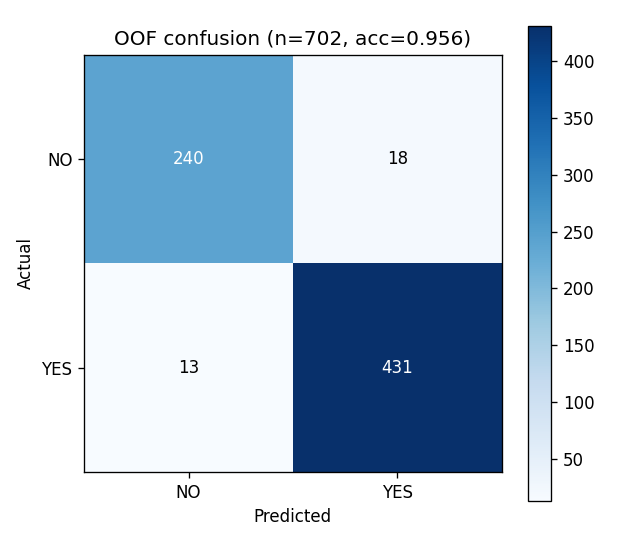
\includegraphics[width=0.85\columnwidth]{confusion_matrix.png}
  \caption{Out-of-fold confusion matrix aggregated over all five folds.
    Accuracy: \SI{95.6}{\percent}. Rows are ground truth, columns are
    predictions.}
  \label{fig:cm}
\end{figure}

\begin{table}[t]
  \centering
  \small
  \caption{Per-fold held-out accuracy and confusion matrices.}
  \label{tab:folds}
  \begin{tabular}{ccccc}
    \toprule
    Fold & Acc. & TN & FP & FN\,/\,TP \\
    \midrule
    1 & 0.957 & 49 & 3 & 3\,/\,86 \\
    2 & 0.965 & 48 & 4 & 1\,/\,88 \\
    3 & 0.986 & 51 & 1 & 1\,/\,87 \\
    4 & 0.943 & 46 & 5 & 3\,/\,86 \\
    5 & 0.929 & 46 & 5 & 5\,/\,84 \\
    \bottomrule
  \end{tabular}
\end{table}

Per-fold accuracy (Table~\ref{tab:folds}) ranges from \num{0.929} to
\num{0.986}. The aggregate out-of-fold confusion matrix
(Figure~\ref{fig:cm}) yields precision/recall of
\num{0.960}\,/\,\num{0.971} for the \textsc{yes} class and
\num{0.949}\,/\,\num{0.930} for the \textsc{no} class (F1 \num{0.965}
and \num{0.939} respectively). Because the downstream ordinance
heuristics are integrated over hours and days, the per-clip error
floor of ${\sim}\SI{4.4}{\percent}$ contributes at most a few units
of bias to hourly bark counts, well below the thresholds used below.

% -----------------------------------------------------------------------
\section{Scoring Pipeline}
The offline scorer (\texttt{bark\_report.py}) re-processes every
recording written by the detector. Rather than reusing the
\texttt{librosa} feature extractor from training, it replicates the
log-mel computation on GPU with
\texttt{torchaudio.transforms.MelSpectrogram} and batched
\texttt{power-to-dB(ref=max)}. This is numerically equivalent to the
training-time librosa pipeline to within ${\sim}10^{-3}$\,dB and
reduces end-to-end scoring time for ${\sim}5400$ clips from
${\sim}\SI{90}{s}$ to under \SI{7}{s} on the RTX 5070 Ti.

\paragraph{Parallel I/O.} WAV decoding is parallelized across a
\texttt{ProcessPoolExecutor} of \texttt{n\_cpu} workers using
\texttt{soundfile.read}. Workers hand fixed-length
\texttt{float32} arrays to the main process, which stacks them into
batches of \num{256} and hands them to the GPU. \texttt{tqdm} wraps
the worker output for a live progress bar.

\paragraph{Per-clip bark counter.} A single event can contain between
one and four distinct barks. To estimate the number of barks per clip
the scorer runs a GPU onset counter directly on the raw waveform:
\begin{enumerate}
  \item Compute a \SI{20}{ms} RMS envelope in dB
        (\texttt{F.avg\_pool1d} of $x^2$).
  \item Non-max suppress with a $\pm$\SI{150}{ms} window via
        \texttt{F.max\_pool1d}.
  \item Keep peaks that are (a) within \SI{12}{dB} of the clip's
        loudest frame and (b) above an absolute floor of
        \SI{-45}{dBFS}.
  \item Clip the per-clip count at \num{8} to guard against buzzing.
\end{enumerate}
For clips whose classifier probability is below threshold the estimated
count is forced to zero; for clips above threshold it is
$\max(\text{count},1)$. Across the evaluation window the mean
multiplier is \num{3.00} barks per bark-clip
($5808 / 1933$).

% -----------------------------------------------------------------------
\section{Analysis Framework}
Filenames record UTC. The reporter converts each timestamp to
\texttt{America/Denver} local time via \texttt{zoneinfo} before any
aggregation so that hourly statistics align with the local day. Events
with classifier probability below \num{0.10} are dropped from the
aggregates to prevent low-confidence detector triggers from dominating
the bar charts; events on explicitly excluded dates are also removed.

\paragraph{Ordinance heuristics.} Fort Collins \S~4-94 defines
``unreasonable noise'' qualitatively via (i) time of day, (ii) duration,
(iii) noise level, and (iv) other disruptive factors. It prescribes no
numeric thresholds and requires a citizen affidavit. The reporter
applies the following configurable heuristics to flag candidate
violations:

\begin{center}
\small
\begin{tabular}{ll}
\toprule
Heuristic & Threshold \\
\midrule
Night hours            & 22:00\,--\,07:00 local \\
Day hourly level       & $\geq$\,\num{20} barks/hr \\
Night hourly level     & $\geq$\,\num{5} barks/hr \\
Sustained duration     & $\geq$\,\num{3} consecutive hrs @ \num{5}+/hr \\
Daily total            & $\geq$\,\num{100} barks \\
\bottomrule
\end{tabular}
\end{center}

These thresholds are defaults exposed as CLI flags; they are not a
legal finding.

% -----------------------------------------------------------------------
\section{Results}
Across the \num{13}-day evaluation window (April 8\,--\,20, 2026, local)
the scorer processed \num{5385} raw detector events. \num{2278}
survived the minimum-confidence filter; of these \num{1933} were
classified as barks, and the GPU onset counter estimated \num{5808}
distinct barks in total. All \num{13} days exceeded one or more of the
ordinance heuristics.

\begin{figure*}[t]
  \centering
  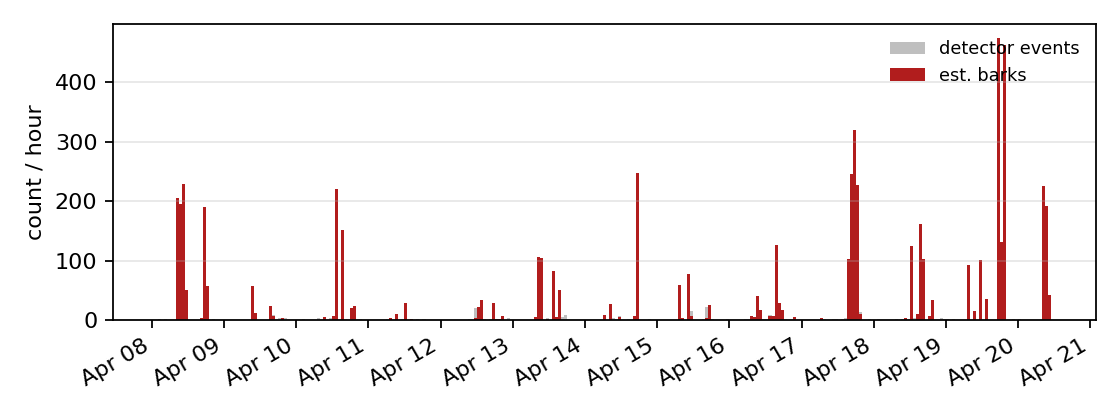
\includegraphics[width=0.98\textwidth]{fig_timeline.png}
  \caption{Hourly bark activity over the full evaluation window, local
    time (\texttt{America/Denver}). Grey: detector events; red:
    estimated barks. Each tick is one local midnight.}
  \label{fig:timeline}
\end{figure*}

The hourly timeline (Figure~\ref{fig:timeline}) shows strong
concentration during daylight hours with a conspicuous weekend peak.
Aggregating over days (Figure~\ref{fig:hour}\textsc{a}) localizes the
peak of the day between \num{14}:00 and \num{18}:00 local.
The day-of-week $\times$ hour view
(Figure~\ref{fig:hour}\textsc{b}) isolates Sunday \num{17}:00 as the
worst cell: \num{502} estimated barks.

\begin{figure}[t]
  \centering
  \begin{subfigure}[b]{\columnwidth}
    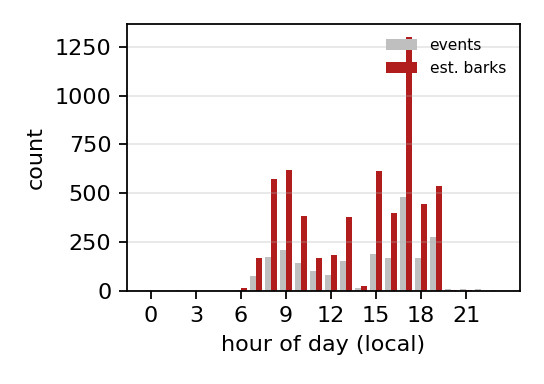
\includegraphics[width=\columnwidth]{fig_hour_hist.png}
    \caption{Totals by hour of day.}
  \end{subfigure}\\[3pt]
  \begin{subfigure}[b]{\columnwidth}
    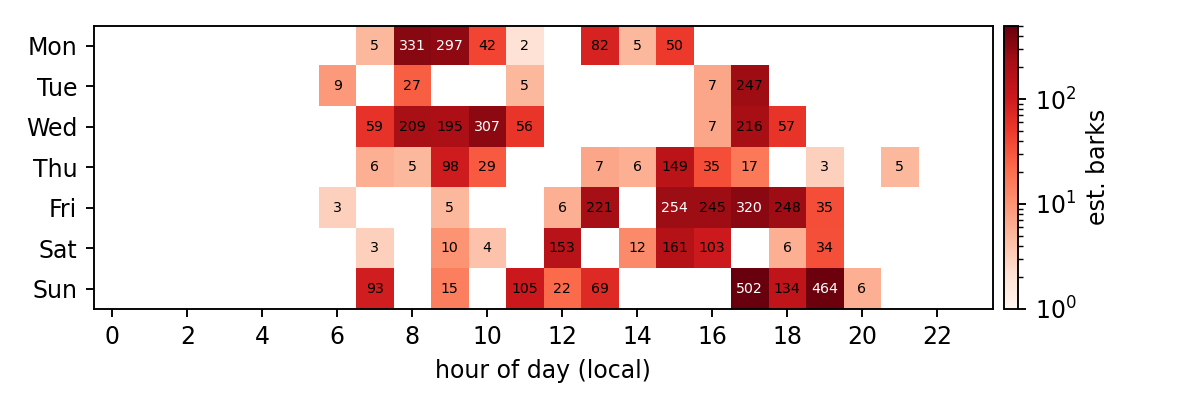
\includegraphics[width=\columnwidth]{fig_dow_hour.png}
    \caption{Day-of-week $\times$ hour heatmap (log color scale).}
  \end{subfigure}
  \caption{Hour-of-day aggregates. (\textsc{a}) shows detector events
    (grey) versus estimated barks (red). (\textsc{b}) shows estimated
    barks only.}
  \label{fig:hour}
\end{figure}

\begin{figure*}[t]
  \centering
  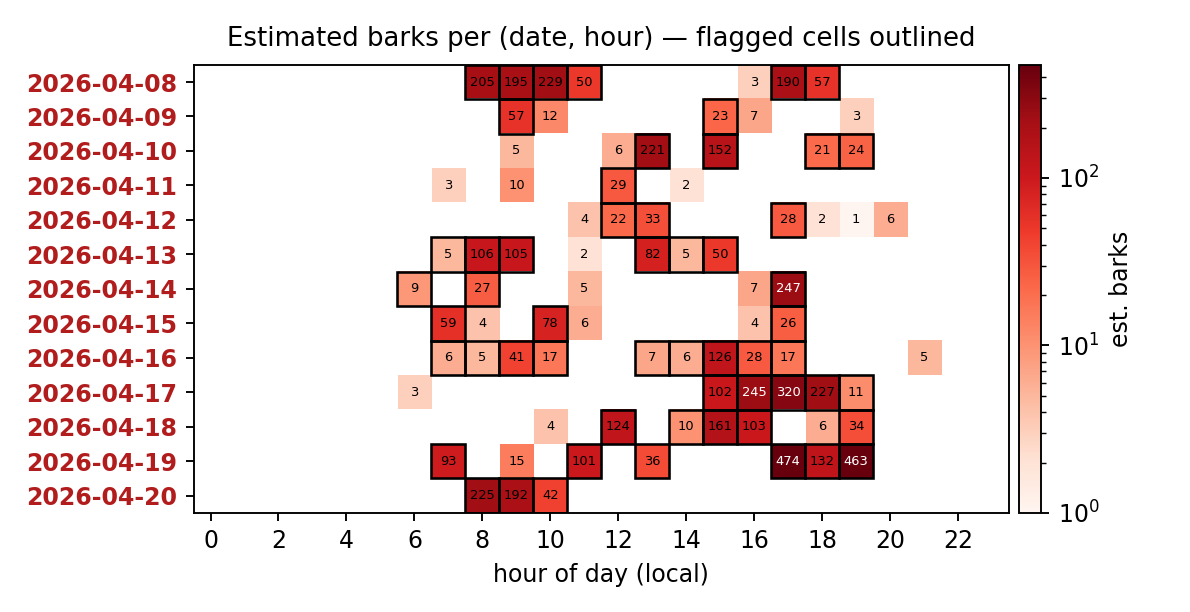
\includegraphics[width=0.98\textwidth]{fig_date_hour.png}
  \caption{Estimated barks per (date, hour) cell. Color: log-scaled
    bark count. Black outlines: cells flagged under the \S~4-94
    heuristics. Red bold y-axis labels: dates flagged at the
    day level.}
  \label{fig:date_hour}
\end{figure*}

The full date $\times$ hour heatmap (Figure~\ref{fig:date_hour})
visualizes which cells exceed the heuristics. The worst day in the
window is Sunday April 19 with \num{1314} estimated barks across
\num{11} flagged hourly cells; the quietest flagged day
(Thursday April 9) still exceeds the day-hourly-level heuristic.

% -----------------------------------------------------------------------
\section{Limitations}

\paragraph{Single-dog assumption.} The classifier is trained on one
dog's bark captured through one microphone. Recalibrating for a
different setting requires re-labeling and, likely, retuning the
band-pass filter.

\paragraph{Bark-count heuristics.} The GPU onset counter operates on
the raw waveform, not on source-separated audio. In overlapping events
(a bark during a car horn, for example) it may over-count; during
wind gusts of similar spectral shape it may fire spuriously on
waveform peaks that the classifier subsequently suppresses only when
the full clip is considered.

\paragraph{Ordinance mapping.} \S~4-94 is adjudicated subjectively and
requires a sworn citizen affidavit. The heuristics here are a
quantitative proxy for the qualitative factors the ordinance lists;
they are not a legal finding and are not presented as evidence.

\paragraph{Clock.} Filenames encode UTC and conversion to local time
crosses the DST boundary cleanly, but any hours missing from the
detector log (service restart, power outage) will appear as zero in
the aggregates rather than as an explicit gap marker.

% -----------------------------------------------------------------------
\section{Reproducibility}
All scripts, configuration, and labeled data live in a single
self-contained directory. The relevant entry points are:
\begin{itemize}
  \item \texttt{bark\_detector.py} --- capture daemon (systemd-managed).
  \item \texttt{label\_barks.py} --- labeling UI.
  \item \texttt{train\_bark\_cnn.py} --- CV training and production fit.
  \item \texttt{bark\_report.py} --- offline scoring and analysis.
  \item \texttt{report\_figures.py} --- generator for this report's
        figures.
\end{itemize}
Dependencies are pinned in the local \texttt{venv} and include
\texttt{torch 2.11}, \texttt{torchaudio 2.11}, \texttt{librosa 0.11},
\texttt{scikit-learn 1.8}, and \texttt{paho-mqtt}.

\end{document}
